\section{Alternative Path Planner}
\label{app:path_planner}

A digital model of the robot's task space and state configuration is used to generate trajectories to run on the physical robot. A random trajectory is generated by selecting a random point in the robot's task space and using A* to solve for a path between the current end effector position and the target point. A noise map is generated using Perlin noise \cite{perlin_noise} and used as a cost map in the A* algorithm to add task space variations in generated trajectories. The solution path from A* in discretized task space is converted to joint space using the baseline inverse kinematic model. A continuous-time joint trajectory is found using a similar method as \cite{8772208} to ensure $C^4$ smoothness. $C^4$ smoothness is required for exact reproducibility of desired trajectories, as well as helps prevent structural oscillations and requires less energy \cite{8772208}. A sample of this process is shown in Figure \ref{fig:trajectory_generation}. This trajectory is sampled at a given command frequency and is used to set the reference motor velocities in the PID controller. This same method can be used to generate test trajectories consisting of a square, a circle, a sinusoidal pattern, and a zig-zag. 

\begin{figure}[h]
    \centering
    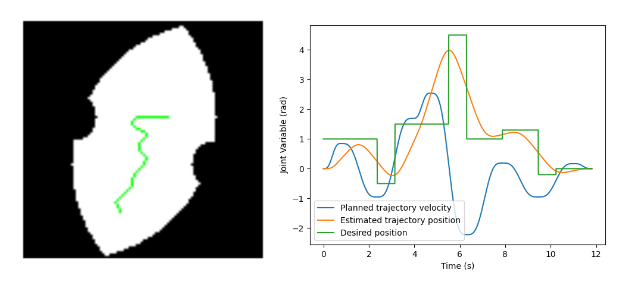
\includegraphics[width=\textwidth]{images/trajectory_generation.png}
    \caption{Trajectory A* search (left) and joint interpolation (right) results}
    \label{fig:trajectory_generation}
\end{figure}